\documentclass[preprint,12pt,authoryear]{elsarticle}
\usepackage[utf8]{inputenc}
\usepackage[T1]{fontenc}
\usepackage{amsmath}
% Times for text and mathematics: the PDF and the Word copy (Times New Roman) share one typeface
\usepackage{mathptmx}
\usepackage{graphicx}
\usepackage{booktabs}
\usepackage{tabularx}
\usepackage{enumitem}
\usepackage[hidelinks]{hyperref}
\usepackage{url}
\setlist{nosep,leftmargin=*}
% let floats stand near their first mention (the defaults pushed Tables 3 and 4 pages away)
\renewcommand{\topfraction}{0.9}
\renewcommand{\bottomfraction}{0.6}
\renewcommand{\textfraction}{0.1}
\renewcommand{\floatpagefraction}{0.75}
\setcounter{topnumber}{3}
\setcounter{totalnumber}{4}
% generated by src/paper/numbers3.py; do not edit
\newcommand{\nSitesDev}{39} % source: results/dev/need2.csv
\newcommand{\nSitesDevFour}{38} % source: results/dev/need2.csv
\newcommand{\nDaysDevAll}{12,674} % source: results/dev/need2.csv
\newcommand{\nDaysDevFour}{10,342} % source: results/dev/need2.csv
\newcommand{\nSitesConf}{36} % source: results/confirm2/need2.csv
\newcommand{\nSitesConfFour}{36} % source: results/confirm2/need2.csv
\newcommand{\nDaysConfFour}{11,133} % source: results/confirm2/need2.csv
\newcommand{\nDaysRetestFour}{11,168} % source: results/retest2024/need2.csv
\newcommand{\needMedConf}{27} % source: results/confirm2/stats_rq1.csv
\newcommand{\needMedConfCI}{27 to 33} % source: results/confirm2/stats_rq1.csv
\newcommand{\needMedConfHi}{33} % source: results/confirm2/stats_rq1.csv
\newcommand{\needPninetyConf}{54} % source: results/confirm2/stats_rq1.csv
\newcommand{\needPnnConf}{132} % source: results/confirm2/stats_rq1.csv
\newcommand{\needMaxConf}{306} % source: results/confirm2/need2.csv
\newcommand{\valueShareConf}{2.34\%} % source: results/confirm2/stats_rq1.csv
\newcommand{\byteShareConf}{4.33\%} % source: results/confirm2/stats_rq1.csv
\newcommand{\oneMsgConf}{7.0\%} % source: results/confirm2/stats_rq1.csv
\newcommand{\needMedDev}{27} % source: results/dev/need2.csv
\newcommand{\needMedRetest}{24} % source: results/retest2024/need2.csv
\newcommand{\shareFiveDev}{0.78\%} % source: results/dev/need2.csv
\newcommand{\shareFifteenDev}{2.34\%} % source: results/dev/need2.csv
\newcommand{\shareSixtyDev}{12.5\%} % source: results/dev/need2.csv
\newcommand{\monthMaxConf}{0.956} % source: results/confirm2/cohort_exact.csv
\newcommand{\monthMinConf}{0.820} % source: results/confirm2/cohort_exact.csv
\newcommand{\gCodeIidConf}{0.900} % source: results/confirm2/stats_rq3.csv
\newcommand{\gCodeIidConfCI}{0.868 to 0.928} % source: results/confirm2/stats_rq3.csv
\newcommand{\dRepIidConf}{0.101} % source: results/confirm2/stats_rq3.csv
\newcommand{\dRepIidConfCI}{0.085 to 0.118} % source: results/confirm2/stats_rq3.csv
\newcommand{\dRepBurConf}{0.026} % source: results/confirm2/stats_rq3.csv
\newcommand{\dRepBurConfCI}{0.021 to 0.031} % source: results/confirm2/stats_rq3.csv
\newcommand{\dRepBsixConf}{0.006} % source: results/confirm2/stats_rq3.csv
\newcommand{\dRepBsixConfCI}{0.005 to 0.007} % source: results/confirm2/stats_rq3.csv
\newcommand{\dFixedIidConf}{0.120} % source: results/confirm2/stats_rq3.csv
\newcommand{\dFixedIidConfCI}{0.093 to 0.152} % source: results/confirm2/stats_rq3.csv
\newcommand{\dRelIidConf}{0.788} % source: results/confirm2/stats_rq3.csv
\newcommand{\dTagIidConf}{0.869} % source: results/confirm2/stats_rq3.csv
\newcommand{\dEveryIidConf}{0.881} % source: results/confirm2/stats_rq3.csv
\newcommand{\gTwelveIidConf}{0.987} % source: results/confirm2/stats_rq3.csv
\newcommand{\gTwelveBurConf}{0.966} % source: results/confirm2/stats_rq3.csv
\newcommand{\regretFixedDev}{0.108} % source: results/dev/robust_regret.csv
\newcommand{\mismatchMaxDev}{0.272} % source: results/dev/robust_mismatch.csv
\newcommand{\tagPolicyDev}{0.103} % source: results/dev/robust_bytes.csv
\newcommand{\tagContentDev}{0.593} % source: results/dev/robust_bytes.csv
\newcommand{\interleaveDev}{0.107} % source: results/dev/robust_bytes.csv
\newcommand{\sitesSixIidConf}{22 of 36} % source: results/confirm2/stats_rq2.csv
\newcommand{\sitesSixBurConf}{5 of 36} % source: results/confirm2/stats_rq2.csv
\newcommand{\sitesTwelveIidConf}{35 of 36} % source: results/confirm2/stats_rq2.csv
\newcommand{\sitesTwelveBurConf}{35 of 36} % source: results/confirm2/stats_rq2.csv
\newcommand{\sizeSuffConf}{83.2\%} % source: results/confirm2/stats_rq4.csv
\newcommand{\sizeSuffConfCI}{75.4\% to 90.4\%} % source: results/confirm2/stats_rq4.csv
\newcommand{\sizePilotsConf}{398} % source: results/confirm2/stats_rq4.csv
\newcommand{\sizeOverConf}{0.3\%} % source: results/confirm2/stats_rq4.csv
\newcommand{\sizeDecConf}{65\%} % source: results/confirm2/stats_rq4.csv (worst month: December)
\newcommand{\rotBsixDev}{0.800} % source: results/dev/multiday.csv
\newcommand{\dailyBsixDev}{0.769} % source: results/dev/multiday.csv
\newcommand{\rotGoneDev}{0.245} % source: results/dev/multiday.csv
\newcommand{\droppedDev}{3,018} % source: results/dev/multiday_summary.csv
\newcommand{\decDOConf}{0.966} % source: results/confirm2/env_summary.csv
\newcommand{\decDOEventConf}{0.737} % source: results/confirm2/env_summary.csv
\newcommand{\eventsDOConf}{750} % source: results/confirm2/env_summary.csv
\newcommand{\decDOEveryConf}{0.160} % source: results/confirm2/env_summary.csv
\newcommand{\decDOTagConf}{0.048} % source: results/confirm2/env_summary.csv
\newcommand{\missECConf}{0.166} % source: results/confirm2/env_summary.csv
\newcommand{\eventsECConf}{766} % source: results/confirm2/env_summary.csv
\newcommand{\missECEveryConf}{0.717} % source: results/confirm2/env_summary.csv
\newcommand{\missECTagConf}{0.679} % source: results/confirm2/env_summary.csv
\newcommand{\missPHConf}{0.372} % source: results/confirm2/env_summary.csv
\newcommand{\eventsPHConf}{392} % source: results/confirm2/env_summary.csv
\newcommand{\missPHEveryConf}{0.163} % source: results/confirm2/env_summary.csv
\newcommand{\glitchCostDev}{2.4} % source: results/dev/robust9_glitch.csv
\newcommand{\corrNoneConf}{0.915} % source: results/confirm2/robust9_corrupt.csv
\newcommand{\corrBerThreeConf}{0.821} % source: results/confirm2/robust9_corrupt.csv
\newcommand{\falseCertConf}{96} % source: results/confirm2/robust9_corrupt.csv
\newcommand{\nDaysCorrConf}{357} % source: results/confirm2/robust9_corrupt.csv (sampled test days)
\newcommand{\crcChecksConf}{148,146} % source: results/confirm2/robust9_corrupt.csv (decoding attempts + rejected data units)
\newcommand{\collisionsExpConf}{2.3} % source: CRC checks / 2^16
\newcommand{\falseCertPostConf}{0} % source: results/confirm2_posthoc2/robust9_corrupt.csv
\newcommand{\falseCertPostDev}{0} % source: results/dev_posthoc2/robust9_corrupt.csv
\newcommand{\postCostThreeConf}{0.037} % source: results/confirm2{,_posthoc2}/robust9_corrupt.csv (Q = 6)
\newcommand{\postCodeTwoConf}{0.066} % source: results/confirm2{,_posthoc2}/robust9_corrupt.csv (Q = 6)
\newcommand{\postRepTwoConf}{0.085} % source: results/confirm2{,_posthoc2}/robust9_corrupt.csv (Q = 6)
\newcommand{\opsFifteenDev}{14,416} % source: results/dev/bench_resources.csv
\newcommand{\opsFiveDev}{134,166} % source: results/dev/bench_resources.csv
\newcommand{\mcuFiveDev}{0.56} % source: 200 cycles per update at 48 MHz
\newcommand{\gCodeIidRetest}{0.908} % source: results/retest2024/stats_rq3.csv
\newcommand{\inwsDays}{24} % source: results/lowcost2/need2.csv
\newcommand{\inwsMedBytes}{64} % source: results/lowcost2/need2.csv
\newcommand{\inwsCodeSix}{0.437} % source: results/lowcost2/cohort_exact.csv
\newcommand{\inwsRepSix}{0.291} % source: results/lowcost2/cohort_exact.csv
\newcommand{\inwsCodeTwelve}{0.763} % source: results/lowcost2/cohort_exact.csv
\newcommand{\inwsRepTwelve}{0.582} % source: results/lowcost2/cohort_exact.csv
\newcommand{\weijaDays}{74} % source: results/lowcost2/plans/Weija.pkl (private data; derived count)
\newcommand{\weijaMedBytes}{27} % source: results/lowcost2/need2.csv
\newcommand{\weijaCodeSix}{0.936} % source: results/lowcost2/plans/Weija.pkl (exact)
\newcommand{\weijaRepSix}{0.837} % source: results/lowcost2/plans/Weija.pkl (exact)
\newcommand{\chainPairsDev}{380} % source: results/dev/e2_anchor_Q6.csv (Q = 6, p = 0.3)
\newcommand{\chainSaveDev}{0.8} % source: results/dev/e2_anchor_Q6.csv (Q = 6, p = 0.3)
\newcommand{\chainGainLoDev}{0.03} % source: results/dev/e2_anchor_Q6.csv (Q = 6, p = 0.3)
\newcommand{\chainGainHiDev}{0.09} % source: results/dev/e2_anchor_Q6.csv (Q = 6, p = 0.3)
\newcommand{\pilotLossDev}{0.061} % source: results/dev/robust_pilot.csv (Q = 6)
\newcommand{\nDaysConfFewer}{1,247} % source: results/confirm2/need2.csv
\newcommand{\needMedConfFewer}{21} % source: results/confirm2/need2.csv
\newcommand{\needSiteEqConf}{30} % source: results/confirm2/need2.csv (median of site medians)
\newcommand{\gSiteMinConf}{0.627} % source: results/confirm2/cohort_exact.csv (site means)
\newcommand{\gSiteMedConf}{0.920} % source: results/confirm2/cohort_exact.csv (site means)
\newcommand{\gSiteMaxConf}{0.989} % source: results/confirm2/cohort_exact.csv (site means)
\newcommand{\gCodeIidBlockCI}{0.885 to 0.913} % source: results/confirm2/stats_rq3.csv (site x month blocks)
\newcommand{\hostFiveS}{4.9} % source: results/dev/bench_resources.csv (table-free, Python)
\newcommand{\hostFiveKB}{43} % source: results/dev/bench_resources.csv
\newcommand{\hostFifteenS}{0.54} % source: results/dev/bench_resources.csv
\newcommand{\hostFifteenKB}{16} % source: results/dev/bench_resources.csv
\newcommand{\hostTableFiveS}{11.9} % source: results/dev/bench_resources.csv (reference table encoder)
\newcommand{\hostTableFiveMB}{8.1} % source: results/dev/bench_resources.csv
\newcommand{\progLines}{7,300} % source: src/{p3,data,paper}/*.py
\newcommand{\nTests}{95} % source: tests/test_*.py (test functions; parametrised cases counted once)

% primitive input, expandable inside tabularx (\input is not)
\makeatletter\newcommand{\tableinput}[1]{\@@input #1 }\makeatother

\journal{Environmental Modelling \& Software}

\begin{document}
\begin{frontmatter}

\title{A regulatory-grade river water-quality record in a few satellite messages a day}

\author[ug]{Kofi Sarpong Adu-Manu\corref{cor}}
\author[ug]{Stephen Kwaku Azongo}
\cortext[cor]{Corresponding author.}
\affiliation[ug]{organization={Department of Computer Science, University of Ghana},
  city={Legon, Accra}, country={Ghana}}

\begin{abstract}
Satellite Internet of Things services reach remote rivers but sell only a few short, one-way messages per day. This study developed a framework that delivers continuous water-quality records within the accuracy that the U.S. Geological Survey (USGS) requires of an excellent record and lets the server certify, from the received bytes alone, which readings meet that tolerance. A node sends the fewest values that keep every reading within tolerance, in 23-byte messages protected by an erasure code sized to each day's record; this choice is optimal among linear designs without knowledge of the loss process. After development on 39 USGS sites, the frozen framework was confirmed on 36 sealed sites in five other regions. A four-parameter day needed a median of two messages. With six messages per day and 30\% simulated loss, the server fully certified \gCodeIidConf{} of days, ahead of repetition, a fixed code, and satellite-tag practice; twelve messages per day certified \gTwelveIidConf{}. Certified records never gave a wrong certain decision and caught conductance pulses that periodic telemetry missed, but did not resolve features finer than the tolerance. Six of eight confirmatory hypotheses held.
\end{abstract}

\begin{keyword}
water-quality monitoring \sep satellite Internet of Things \sep error-bounded records \sep erasure coding \sep data certification \sep reproducible evaluation
\end{keyword}


\end{frontmatter}

\section{Introduction}
\label{sec:intro}

Continuous water-quality monitoring underpins the management of rivers that supply drinking water and receive pollution. In-situ sensors now measure temperature, specific conductance, dissolved oxygen, and pH every few minutes, and the resulting high-frequency records reveal diel cycles, storm responses, and short pulses that grab samples miss \citep{rode2016}. Wireless sensor networks have made such monitoring affordable \citep{adumanu2017}, and deployments in Ghana and Kosovo have shown that it works in practice, but they relied on cellular backhaul \citep{adumanu2020,ahmedi2022}. The rivers under the greatest pressure are often the furthest from that infrastructure; in Ghana, for example, small-scale gold mining has degraded rivers in forested catchments where terrestrial coverage is sparse \citep{duncan2020}. This motivating case is not evaluated here.

Satellite Internet of Things (IoT) services now reach such sites with small, low-power terminals \citep{centenaro2021}, but their capacity is sold in messages, not bandwidth. A typical module sends one-way messages with a payload of 23 bytes and receives no acknowledgement \citep{kineis2023kim1}. A four-parameter sensor sampling every 10 minutes produces 576 readings a day; even packed at 13 bits each, without timestamps, into the 20 bytes that remain after a three-byte message header, they would fill at least 47 messages. A monitoring agency therefore needs to know what a credible record of a river costs, how to deliver it when messages are scarce and may be lost without notice, and what the delivered record can be trusted for. Many uses of such records tolerate a delay of a day: compliance assessment, trend analysis, and model calibration work from daily or longer summaries, whereas alarms that require action within minutes are outside the scope of this study.

This study defined credibility by established practice: a record is sufficiently accurate when every reconstructed reading lies within the tolerance that the USGS requires of an excellent continuous record \citep{wagner2006}. Because the link returns nothing, the server must be able to establish from the bytes it received which readings meet that tolerance. The study asked four research questions:
\begin{enumerate}
  \item RQ1: How many values and messages does a record within tolerance require per day, and how does that need vary across rivers, seasons, and sampling intervals?
  \item RQ2: Which delivery design maximises the share of days that the server can fully certify over a one-way link, without knowledge of the loss process, compared with the designs used in practice?
  \item RQ3: Which message plans suffice, and can an adequate plan be chosen from a short pilot record?
  \item RQ4: Do the delivered records support the decisions that agencies take, such as detecting low dissolved oxygen or conductance pulses?
\end{enumerate}

The algorithms used are established: minimum-size piecewise-linear approximation within a maximum error \citep{imai1988}, budgeted compression of sensor history \citep{deligiannakis2007}, and erasure codes \citep{reed1960}. Satellite-linked animal tags have long sent compressed profiles pseudo-randomly over a one-way link \citep{boehme2009,photopoulou2015}. What had not been established is how these elements must be adapted and combined so that a server without feedback can certify an environmental record, what such a record costs on real rivers, and which decisions it supports. The contributions of this study are the following:
\begin{itemize}
  \item A framework that delivers error-bounded river records over one-way, message-priced links: a quantisation-exact, self-contained encoder; a byte-level message frame; a record-first erasure code; and a server-side certificate that is provably sound and needs no feedback.
  \item A proof that the record-first code maximises the probability of full certification among unit-level linear designs for every loss process, such that it needs no channel knowledge, with exact delivery probabilities that agree with byte-level simulation.
  \item An evaluation on \nSitesDev{} development sites and \nSitesConf{} sealed confirmation sites in five other regions, with the software and analysis plan frozen before the confirmation data were opened.
  \item A decision-oriented assessment: certified records never gave a wrong certain decision and detected short events that periodic and tag telemetry missed, but they do not resolve features finer than the tolerance.
\end{itemize}

Section~\ref{sec:related} reviews related work. Section~\ref{sec:model} describes the framework. Section~\ref{sec:study} describes the data and the study design. Section~\ref{sec:results} reports the results, Section~\ref{sec:discussion} discusses them, and Section~\ref{sec:conclusion} concludes.

\section{Related work}
\label{sec:related}

\subsection{Error-bounded reduction of sensor records}
Sensor data reduction with guaranteed accuracy has two classical formulations. The first fixes a precision and minimises communication: \citet{olston2003} adapted per-source filter widths so that continuous queries met their precision constraints with the fewest updates, and \citet{deligiannakis2004} redistributed error thresholds within aggregation trees. The second fixes a budget and minimises error. Self-based regression (SBR) compresses the buffered multi-signal history of a sensor node to a bandwidth budget and supports a maximum-absolute-error objective; in its localised mode, a group leader repeatedly allocates residual bandwidth to the member with the largest error \citep{deligiannakis2007}. For a single signal, the fewest vertices of a piecewise-linear approximation within a maximum error can be found in linear time \citep{imai1988}, also online \citep{soroush2008}, and many signals can be archived jointly under one maximum error \citep{gandhi2009}. Storage-side work has produced multi-resolution summaries for drill-down queries \citep{ganesan2003}, predictive archival with on-demand retrieval \citep{desnoyers2005}, and layered time-series encodings that decode at several error levels \citep{barbarioli2023}. This study used the minimum-size approximation as its node encoder. It did not propose a new compression algorithm; it measured what that encoder costs for regulatory tolerances on rivers, and how its output survives a link without acknowledgements, which these works assume to be reliable.

\subsection{Satellite IoT and one-way delivery}
Direct-to-satellite IoT has been studied mainly at the medium-access layer: constellation design for revisit time \citep{capez2022}, slotted ALOHA with erasures at several satellites \citep{tondo2021}, uplink transmission policies \citep{alvarez2022}, scheduling of LoRa uplinks to passing satellites \citep{afhamisis2022}, and message replication for reliability \citep{rathi2025}. These works treat packets as interchangeable and do not address what the packets should contain. Terrestrial schemes for bulk transfer of buffered data aim to deliver every byte \citep{abdelfadeel2020}. The closest practice to this study comes from animal telemetry. Conductivity–temperature–depth satellite relay data loggers abstract each ocean profile to a fixed number of points, store the resulting messages in a buffer, and send them pseudo-randomly through the one-way Argos system so that losses are spread over an unbiased sample \citep{boehme2009,photopoulou2015}. That practice fixes the number of points, not the accuracy, and it was included in this study as a baseline.

\subsection{Freshness and value of information}
A large literature optimises the age or value of the information held about the current state of a source \citep{yates2021}, including over random-access and satellite links \citep{chen2021,talli2026,ramachandran2026}. These models keep only the newest sample of a synthetic process; \citet{chen2021}, for example, assumed a one-packet buffer in which new packets replace older ones. Environmental regulation needs the whole record, not only its latest value, which is why this study used a record-wide maximum error as its objective. A record within tolerance everywhere also holds the latest value within tolerance.

\section{Framework}
\label{sec:model}

Fig.~\ref{fig:arch} summarises the framework. A sensor node at a remote river site records several water-quality parameters. At the end of each day it selects the fewest readings from which the server can reconstruct every reading within a tolerance, packs them into messages, and adds redundancy. The satellite link delivers each message or loses it, and the node never learns which. The server decodes what arrived, reconstructs the record, and states which readings it can certify; agencies then take decisions that use only certified readings.

\begin{figure}[t]
\centering
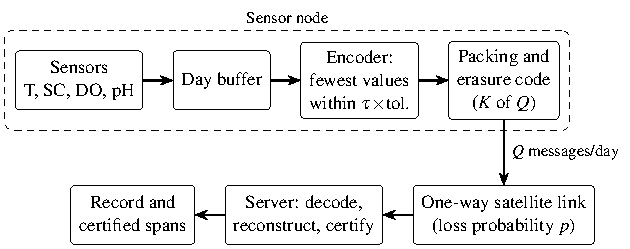
\includegraphics[width=\textwidth]{figs/arch.pdf}
\caption{Workflow of the framework. The node never learns which messages arrived; the server uses only the bytes that arrived and the site profile (the sampling interval of each parameter).}
\label{fig:arch}
\end{figure}

\subsection{Record, tolerance, and reconstruction}
\label{sec:record}
A channel-day is one parameter $j$ of one site on one UTC day, with readings $x_j(t)$, $t = 0, \dots, n_j - 1$, on the parameter's own sampling grid. Each reading has a tolerance $\delta_j(t) > 0$. This study used the accuracy that the USGS requires of an excellent continuous record \citep{wagner2006}: 0.2\,\textdegree C for temperature, 3\% of the value for specific conductance, the greater of 0.3\,mg/L and 5\% of the value for dissolved oxygen, and 0.2 units for pH. The tolerance is relative to the sensor record; the accuracy of the sensor itself (calibration, fouling, and drift) is outside it.

The node quantises a kept reading to a 13-bit code (Section~\ref{sec:frame}), and the server holds the dequantised value $\tilde{x}_j(s)$. From the kept slots that reached it, $s_1 < \dots < s_k$, the server reconstructs $\hat{x}_j(t)$ by holding $\tilde{x}_j(s_1)$ back to midnight, interpolating linearly between consecutive kept slots, and holding $\tilde{x}_j(s_k)$ to the end of the day. Each day is therefore self-contained: no value of the previous day is needed. Chaining days, in which each day starts from the previous day's last value, saved \chainSaveDev{} values per day on \chainPairsDev{} pairs of consecutive development days. However, at six messages per day and a loss probability of 0.3, a chained day was fully certified \chainGainLoDev{} to \chainGainHiDev{} less often, because its first span depends on the previous day's final message; bursts across midnight affected it most. The normalised error of a reading is
\begin{equation}
e_j(t) = \frac{|x_j(t) - \hat{x}_j(t)|}{\delta_j(t)}.
\label{eq:err}
\end{equation}

\subsection{Encoder}
\label{sec:encoder}
For a level $\tau$, the encoder selects for each parameter the fewest slots $S_j(\tau)$ whose reconstruction keeps $e_j(t) \le \tau$ for every reading; the record of a day is the union of these sets at $\tau = 1$, listed in a fixed planned order (temperature, dissolved oxygen, pH, specific conductance; then time). Three features make the bound exact and the record self-contained:
\begin{itemize}
  \item Quantisation: every candidate error is computed with the dequantised endpoint values that the server will hold; therefore, the bound includes quantisation and needs no margin.
  \item Head and tail: the first kept value is held back to midnight and the last is held to the end of the day; thus, a flat parameter costs one value and no anchor from the previous day is used.
  \item Censoring: a reading outside the quantiser range (for example a sensor fault reported as a negative concentration) is always kept, carried as its flag code, excluded from the bound, and reported by the server as below or above range.
\end{itemize}
The selection is the minimum-number problem of polygonal approximation \citep{imai1988}, here with per-reading tolerances. It was solved exactly by a forward dynamic program: for a fixed start, a span to a later slot keeps every reading in between within tolerance exactly when the slope of the span lies in the intersection of the slope windows imposed by those readings \citep{orourke1981}, an intersection that only shrinks as the span grows. Head and tail spans are checked with prefix and suffix intervals. The encoder needs $O(n^2)$ time and $O(n)$ memory per channel-day; it reproduced the plans of a reference implementation built on a full error table on all \nDaysDevAll{} record days of the development year.

\subsection{Message frame}
\label{sec:frame}
Each message carries the 23-byte user payload of the KIM1 module \citep{kineis2023kim1}. The operator delivers it with the device identifier and the time of reception at the satellite \citep{kineis2024formats}; neither is in the payload. Table~\ref{tab:frame} provides the layout. A three-byte header identifies the day block, the message, and the number of data units $K$. The remaining 20 bytes form a unit that is protected as a whole by the erasure code. A unit carries a CRC-16 computed over its content and its context (block day, $K$, and unit index), such that a unit recovered from a corrupted or misassociated message is rejected. It then carries up to three segments, each holding consecutive values of one record day with the position of its first value in the planned order. Values carry their parameter, slot, and reading. Linear grids are decimal (0.01\,\textdegree C, 0.005\,mg/L, and 0.002 pH units); thus, readings reported at 0.1 or 0.01 are carried exactly. Specific conductance uses a logarithmic grid whose step is 0.14\% of the value. The worst quantisation error is 2.5\% of the tolerance. A unit holds five values (three in a 19-byte payload); the header and integrity fields take 35\% of the payload.

\begin{table}[t]
\centering
\caption{Message frame (23-byte payload).}
\label{tab:frame}
\small
\begin{tabularx}{\textwidth}{@{}llX@{}}
\toprule
Part & Bits & Fields \\
\midrule
Header (not coded) & 24 & version (2); block day modulo 64 (6); message index (7); $K$ (7); coded (1); code type (1) \\
Unit check & 16 & CRC-16 over the unit and its context \\
Segment count & 2 & 0 to 3 segments \\
Segment header & 21 & day offset from the block day (6); first planned position (10); value count (3); last value of the day (1); record within tolerance (1) \\
Value & 24 & parameter (2); slot (9); reading code (13; codes 0 and 8191 flag a reading below or above range) \\
Padding & & zeros to 20 bytes \\
\bottomrule
\end{tabularx}
\end{table}

The block day is unwrapped from the operator's reception time, which is unambiguous while the delay from sending to reception is below 63 days and the node clock is within one day of UTC. The planned positions let the server know exactly which values it lacks without any feedback.

\subsection{Delivery designs}
\label{sec:designs}
A plan allows $Q$ messages per day. Let $D_1$ be the number of units that the day's record occupies. The proposed design, the record-first code, sends the $D_1$ data units and $Q - D_1$ parity messages of a systematic Reed--Solomon code over GF($2^8$) \citep{reed1960}; any $D_1$ of the $Q$ messages recover the record. $D_1$ changes from day to day and travels in every header. Days whose record exceeds $Q$ units send their first $Q$ units, which yield partial certificates only. Table~\ref{tab:designs} lists the baselines, which use the same frame and quota.

\begin{table}[t]
\centering
\caption{Delivery designs compared (same frame and the same $Q$ messages per day).}
\label{tab:designs}
\small
\begin{tabularx}{\textwidth}{@{}lX@{}}
\toprule
Design & Content and transmission \\
\midrule
Record-first code (proposed) & The record; $D_1$ data units and $Q - D_1$ Reed--Solomon parity messages. \\
Record-first fountain code & The record; $D_1$ data units and $Q - D_1$ random linear combinations over GF($2^8$) \citep{luby2002,ho2006}. \\
Record-first repetition & The record; units sent round robin over all $Q$ messages (copies interleaved); also in block order. \\
Fixed-$K$ code & The fewest values at the smallest level $\tau$ that fills $5K$ values; $K$ data units and $Q - K$ parity; $K$ chosen without knowledge of the channel. \\
Fixed-$r$ repetition & As the fixed-$K$ code for $\lfloor Q / r \rfloor$ units, repeated round robin. \\
Reliable-link design & The fewest values at the smallest $\tau$ that fills $5Q$ values, each unit sent once: optimal when no message is lost \citep{deligiannakis2007}. \\
Tag practice & A fixed number of broken-stick points per parameter (endpoints first, then the largest absolute deviation), with units picked pseudo-randomly with replacement for each transmission, as satellite-linked animal tags do \citep{boehme2009,photopoulou2015}; a seven-day buffer version rotates units over the following week. \\
Every $k$-th reading & Every $k$-th reading of every parameter, newest included, $k$ as small as the quota allows. \\
\bottomrule
\end{tabularx}
\end{table}

\subsection{Decoding and certification}
\label{sec:cert}
The server keeps the majority header of each block, accepts only units that pass their CRC, and decodes the erasure code when sufficient messages arrived, retrying other parity messages if a recovered unit fails its check. It then certifies readings from the received planned positions alone:
\begin{itemize}
  \item a span between two consecutive planned positions of the same parameter is certified when both arrived;
  \item the head of a parameter is certified when its first planned value arrived and is known to be first (position 0, or the preceding position arrived and belongs to another parameter);
  \item the tail is certified when its last planned value arrived and is known to be last (the next position belongs to another parameter, or the segment carries the last-value flag);
  \item censored readings are reported as below or above range and never certified.
\end{itemize}

Proposition 1 (soundness): if the record keeps every reading within tolerance, every value used arrived as transmitted, the block day was unwrapped correctly, the site profile is correct, and each day has one record, then every certified reading satisfies $e_j(t) \le 1$ in Eq.~(\ref{eq:err}). The reconstruction on a certified span depends only on the two received values that bound it, which are the values the encoder used; therefore, the encoder's bound carries over. A day is fully certified exactly when all its planned values arrived.

Proposition 2 (record-first coding needs no knowledge of the channel): among designs whose messages carry linear combinations of the record's $D_1$ units, no design fully certifies a day with probability greater than $P(N \ge D_1)$, where $N$ is the number of messages that arrive, and the record-first code attains this bound for every loss process, including bursty and correlated loss. Recovering $D_1$ unknown units requires at least $D_1$ received combinations, and a maximum-distance-separable code recovers them from any $D_1$ messages.

The study distinguished four quantities, which are easy to conflate:
\begin{itemize}
  \item the record error, $\max e_j(t)$ over the record, which the encoder knows exactly;
  \item full certification, which the server establishes from the received bytes;
  \item the share of days within tolerance as judged by an observer who knows the full sensor record, which includes days that are within tolerance by chance but cannot be verified;
  \item the probability of full certification under a stated loss model, $G_{\mathrm{cert}}$, which is the primary outcome.
\end{itemize}
No design guarantees delivery over a one-way link that loses messages; Proposition 1 guarantees that whatever the server certifies is within tolerance.

\subsection{Decisions from certified records}
\label{sec:decisions}
A certified reading bounds the true reading: because $|x - \hat{x}| \le \delta(x)$ with $\delta(x) = \max(a, r|x|)$ for the constants $a$ and $r$ of each parameter, the server can compute an interval that contains $x$ from $\hat{x}$ alone. For a criterion such as a daily minimum of dissolved oxygen below 5\,mg/L, the server therefore states one of three outcomes: certainly exceeded (some certified interval lies entirely below the threshold), certainly not exceeded (every reading is certified and every interval lies above it), or undetermined. The first two cannot be wrong under the conditions of Proposition 1. Designs without a bound can only compare their reconstruction with the threshold.

\section{Data and study design}
\label{sec:study}

\subsection{Data}
\label{sec:data}
All data were approved instantaneous values from the USGS National Water Information System \citep{usgs2016nwis}; dissolved oxygen was used in mg/L, the unit of the accuracy rating. Each parameter was used on its own sampling grid on each UTC day (5 to 60 minutes); a run of at most two missing readings with valid neighbours on both sides was bridged linearly, and any longer gap made that parameter-day ineligible. A record day carried the parameters that were eligible on that day. The primary cohort consisted of record days with all four parameters. Three data sets were used:
\begin{itemize}
  \item Development: calendar year 2023 at \nSitesDev{} sites in New Jersey, Pennsylvania, Illinois, and Oregon (\nDaysDevFour{} four-parameter days at \nSitesDevFour{} sites). Every design choice and every threshold was set on these data.
  \item Confirmation: calendar year 2024 at \nSitesConf{} sites in five regions that the development sites do not represent (the Southeast, the Mountain West, the Great Plains and upper Midwest, the Southwest and Texas, and New England and New York; \nDaysConfFour{} four-parameter days at \nSitesConfFour{} sites). The sites were drawn at random from those whose USGS series catalogue covered 2024 for all four parameters and which had at least 250 approved daily values of each, using metadata and approval counts only.
  \item Temporal re-test: calendar year 2024 at the development sites (\nDaysRetestFour{} four-parameter days). These data had been opened in an earlier round of this study and are reported as a re-test, not as confirmation.
\end{itemize}
Table~\ref{tab:cohort} summarises the cohorts. Supplementary Tables S1 and S2 list every site, and Supplementary Table S3 provides the flow from parameter-days to record days, including the days with fewer than four parameters.

\begin{table}[t]
\centering
\caption{Cohorts (four-parameter record days; sites with at least one such day).}
\label{tab:cohort}
\small
\begin{tabularx}{\textwidth}{@{}Xrrrr@{}}
\toprule
Cohort & Sites & Days & Main interval & Median days per site \\
\midrule
\tableinput{tables/cohorts.tex}
\bottomrule
\end{tabularx}
\end{table}

\subsection{Loss models and message plans}
\label{sec:channels}
No measured loss rate was available for the target service; therefore, loss was modelled. Independent loss removed each message with probability $p$; a two-state Gilbert channel \citep{gilbert1960,elliott1963} lost every message in its bad state, with the same mean loss $p$ and mean bursts of three or six messages. Loss probabilities from 0.05 to 0.6 were evaluated, within the range studied for direct-to-satellite links \citep{tondo2021}; $p = 0.3$ is the reference. One loss process ran through all messages in order; thus, bursts could span midnight. Plans of 1, 6, 12, 24, and 96 messages per day were evaluated as illustrative tiers.

\subsection{Environmental decision criteria}
\label{sec:criteria}
Four criteria common in regulatory practice were evaluated, with thresholds fixed before any design was compared:
\begin{itemize}
  \item Low dissolved oxygen: a daily minimum below 5.0\,mg/L \citep{epa1986do}.
  \item pH out of range: any reading below 6.5 or above 9.0 \citep{epa1986gold}.
  \item Warm water: a seven-day average of the daily maximum temperature (7DADM) above 20\,\textdegree C \citep{epa2003temp}, a criterion that requires several consecutive days.
  \item Conductance pulse: a change of specific conductance by more than 10\% within one hour, as caused, for example, by a discharge (a criterion defined for this study).
\end{itemize}
For each criterion and day, the reconstruction was read in two ways: naively, by comparing it with the threshold, and with the three-valued rule of Section~\ref{sec:decisions}, using certified readings only. Both were compared with the full sensor record.

\subsection{Development and confirmation}
\label{sec:procedure}
The study proceeded in two stages:
\begin{enumerate}
  \item Development (2023): the framework was developed and tested on the development sites, including the channel-blind parameters of the baselines (chosen by minimax regret over six channels on half of the sampled days) and the threshold of the plan-sizing rule.
  \item Confirmation (2024, new sites): eight hypotheses with numerical thresholds (Table~\ref{tab:hyp}), the analysis plan, and the software were frozen and checksummed, the repository was tagged, and the freeze record was committed; only then were the sealed confirmation data opened, once, after their checksums had been verified.
\end{enumerate}
The confirmation run was interrupted twice by the end of a computing session and resumed with the same frozen command; finished per-site results were reused and none was inspected before the run was complete. An earlier version of the method had been confirmed on the 2024 data of the development sites; because the method changed in response to a review, those data now serve only as a temporal re-test.

\subsection{Outcomes and statistics}
\label{sec:stats}
The primary outcome was $G_{\mathrm{cert}}$, the probability that a day is fully certified at the server (Section~\ref{sec:cert}). For the record-first code and repetition, $G_{\mathrm{cert}}$ of a day depends only on its record size, the plan, and the loss model, and was computed exactly on every day by forward recursions over the channel state; designs whose content depends on the plan were evaluated on a stratified sample of 20 days per site. The exact probabilities agreed with byte-level simulation, in which every message was built, lost, decoded, and certified from its bytes: over 525 combinations of design, plan, and loss model, the mean absolute difference was 0.0014 and the largest 0.011, within the simulation error. Environmental decisions and corruption tests used 20 loss draws per day. Each outcome has its own unit: four-parameter record days for cost, delivery, and decisions (\nDaysConfFour{} on the confirmation sites); 720 sampled days (20 per site) for designs whose content depends on the plan; sites for the 90\% target; site-pilots for plan sizing (\sizePilotsConf{}); and \nDaysCorrConf{} sampled days for the corruption tests.

Days within a site are not independent; therefore, 95\% intervals were obtained from 2,000 bootstrap resamples of sites \citep{field2007}, with differences between designs computed on the same days. A bootstrap over site-by-month blocks, run as a sensitivity analysis for season, gave a narrower interval for the main estimate (\gCodeIidBlockCI{}, against \gCodeIidConfCI{}); site clustering is therefore the conservative choice reported throughout. A hypothesis passed when its interval lay entirely on the stated side of its threshold (Table~\ref{tab:hyp}). The eight hypotheses are reported jointly without adjustment because each threshold is a substantive margin rather than a test of no effect; all other analyses are descriptive.

\begin{table}[t]
\centering
\caption{Confirmatory hypotheses (frozen before the confirmation data were opened) and their outcome on the \nSitesConf{} confirmation sites.}
\label{tab:hyp}
\small
\begin{tabularx}{\textwidth}{@{}l>{\raggedright\arraybackslash}X>{\raggedright\arraybackslash}p{2.4cm}>{\raggedright\arraybackslash}p{3.7cm}l@{}}
\toprule
 & Hypothesis & Threshold & Result (95\% interval) & Outcome \\
\midrule
\tableinput{tables/hypotheses.tex}
\bottomrule
\end{tabularx}
\end{table}

\section{Results}
\label{sec:results}

Unless stated otherwise, results refer to the \nDaysConfFour{} four-parameter days of the \nSitesConf{} confirmation sites, with the development value (\nDaysDevFour{} days at \nSitesDevFour{} sites) for comparison, and intervals are site-clustered 95\% bootstrap intervals.

\subsection{Cost of a record within tolerance (RQ1)}
\label{sec:need}
A four-parameter day needed a median of \needMedConf{} bytes of values (\needMedConfCI{}), that is, nine values or two messages; the development median was the same (\needMedDev{} bytes). The 90th percentile was \needPninetyConf{} bytes, the 99th percentile \needPnnConf{} bytes, and the largest day needed \needMaxConf{} bytes (Fig.~\ref{fig:need}). The record held \valueShareConf{} of the readings and \byteShareConf{} of the bytes of the raw readings (median), and \oneMsgConf{} of days fitted a single message. With each site weighted equally, the median was \needSiteEqConf{} bytes; the \nDaysConfFewer{} record days with one to three parameters needed a median of \needMedConfFewer{} bytes. On the development data, the share of readings kept rose from \shareFiveDev{} at 5-minute sampling to \shareFifteenDev{} at 15 minutes and \shareSixtyDev{} at hourly sampling, because a smooth signal sampled often needs few values, whereas an hourly record leaves little to omit. The need was largest in summer: the share of days fully certified with six messages per day fell from \monthMaxConf{} in winter to \monthMinConf{} in July and August (Supplementary Fig. S1).

\begin{figure}[t]
\centering
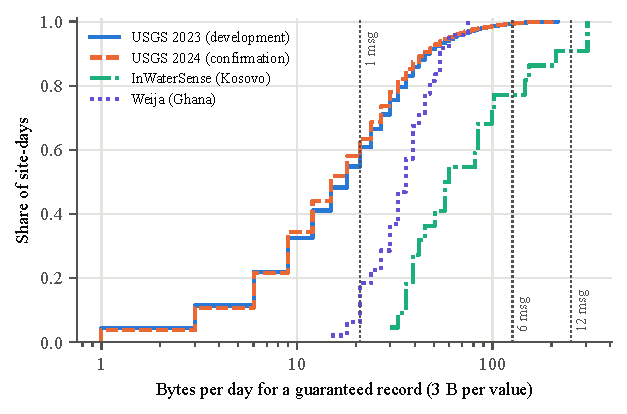
\includegraphics[width=0.6\textwidth]{figs/need_ecdf.pdf}
\caption{Bytes of values needed for a record within tolerance, per four-parameter day. Vertical lines mark the capacity of one, two, and six messages.}
\label{fig:need}
\end{figure}

\subsection{Delivery without knowledge of the channel (RQ2)}
\label{sec:delivery}
Table~\ref{tab:delivery} and Fig.~\ref{fig:delivery} compare the designs at six messages per day. At an independent loss probability of 0.3, the record-first code fully certified \gCodeIidConf{} of days (\gCodeIidConfCI{}); site means ranged from \gSiteMinConf{} to \gSiteMaxConf{}, with a median of \gSiteMedConf{} (Supplementary Table S2). It exceeded record-first repetition by \dRepIidConf{} (\dRepIidConfCI{}), the channel-blind fixed-$K$ code by \dFixedIidConf{} (\dFixedIidConfCI{}), the reliable-link design by \dRelIidConf{}, tag practice by \dTagIidConf{}, and every $k$-th reading by \dEveryIidConf{}. The advantage over repetition shrank as loss became burstier: \dRepBurConf{} (\dRepBurConfCI{}) with bursts of three messages and \dRepBsixConf{} (\dRepBsixConfCI{}) with bursts of six, where both designs lose whole runs of messages whatever they carry. The code was never below repetition on any day, as Proposition 2 requires.

\begin{table}[t]
\centering
\caption{Days fully certified, $G_{\mathrm{cert}}$, at six and twelve messages per day (confirmation sites; 95\% intervals).}
\label{tab:delivery}
\small
\begin{tabularx}{\textwidth}{@{}>{\raggedright\arraybackslash}X*{4}{>{\raggedright\arraybackslash}p{2.3cm}}@{}}
\toprule
Design & Independent, $p = 0.1$ & Independent, $p = 0.3$ & Bursty, $p = 0.3$ & Bursts of 6, $p = 0.3$ \\
\midrule
\tableinput{tables/delivery.tex}
\bottomrule
\end{tabularx}
\end{table}

\begin{figure}[t]
\centering
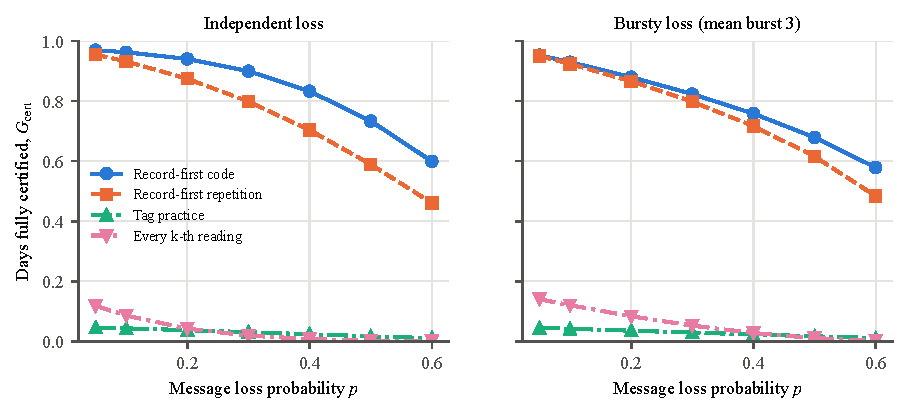
\includegraphics[width=\textwidth]{figs/delivery.pdf}
\caption{Days fully certified against the message loss probability, six messages per day (confirmation sites).}
\label{fig:delivery}
\end{figure}

Three analyses on the development data explain the ranking:
\begin{itemize}
  \item Channel knowledge: a code of fixed dimension needs the loss rate to choose $K$. Chosen without it, it lost up to \regretFixedDev{} against the same code tuned for the true channel; tuned for a loss probability of 0.1 and used at 0.6, it lost \mismatchMaxDev{} (Fig.~\ref{fig:mismatch}). The record-first code was at least as good as the tuned fixed code on all 15 channels and four tiers. A server that estimated the channel from the message indices of a 28-day pilot and reconfigured the node lost at most \pilotLossDev{}: feasible, but unnecessary with record-first coding.
  \item Content versus transmission policy: sending the record's units with the tags' random policy cost \tagPolicyDev{} against interleaved repetition, whereas sending broken-stick points instead of the record cost a further \tagContentDev{}: tag practice lost mainly because its points are not chosen against a tolerance.
  \item Other codes and orders: a systematic random linear (fountain-style) code matched Reed--Solomon to within 0.001; interleaving repetition copies made no difference under independent loss but added \interleaveDev{} under bursty loss.
\end{itemize}

\begin{figure}[t]
\centering
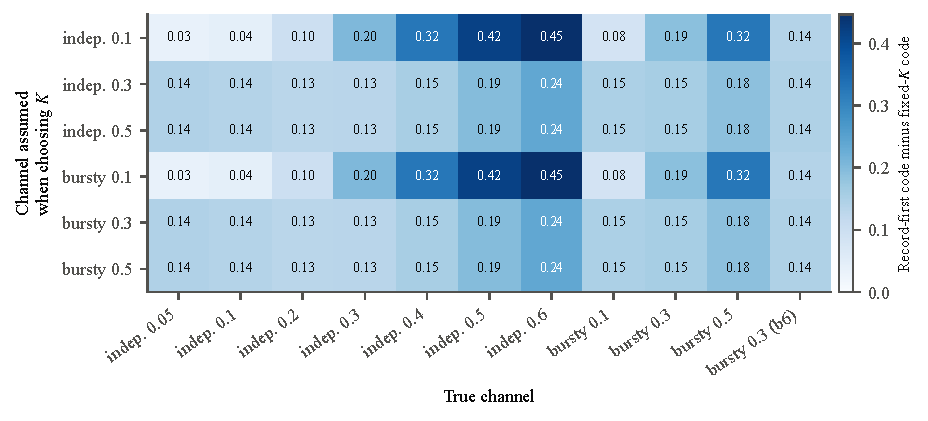
\includegraphics[width=\textwidth]{figs/mismatch.pdf}
\caption{Advantage of the record-first code over a fixed-$K$ code chosen for an assumed channel (rows) and used on the true channel (columns); six messages per day, development data.}
\label{fig:mismatch}
\end{figure}

\subsection{Message plans, buffering, and plan sizing (RQ3)}
\label{sec:plans}
A site met the target when at least 90\% of its days were fully certified within seven days. With six messages per day, \sitesSixIidConf{} confirmation sites met it under independent loss of 0.3 and \sitesSixBurConf{} under bursty loss; with twelve messages, \sitesTwelveIidConf{} and \sitesTwelveBurConf{}; with 24, all. With twelve messages per day, the code certified \gTwelveIidConf{} of days under independent loss and \gTwelveBurConf{} under bursty loss.

Buffering did not help (development data). A node that carried a first-in, first-out backlog of records into later blocks was never better by more than 0.007 than sending each day's record on the next day at six or more messages per day, and at one message per day its backlog grew without bound and \droppedDev{} record days exceeded the frame's 63-day limit. Rotating the units of the last seven days, as satellite tags do, gave time diversity: under bursts of six messages it certified \rotBsixDev{} of days within a week against \dailyBsixDev{} for the next-day code, but only \rotGoneDev{} by the next day (Fig.~\ref{fig:multiday}).

\begin{figure}[t]
\centering
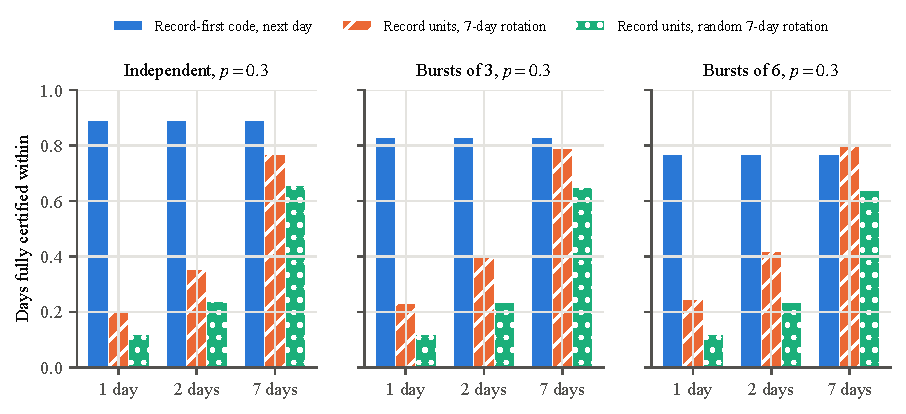
\includegraphics[width=\textwidth]{figs/multiday.pdf}
\caption{Days fully certified within one, two, and seven days for the next-day record-first code and two seven-day rotations of the record's units; six messages per day, development test sites.}
\label{fig:multiday}
\end{figure}

A plan chosen as the smallest tier whose 28-day pilot certified at least 90\% of days within a week was sufficient for the rest of the year in \sizeSuffConf{} (\sizeSuffConfCI{}) of \sizePilotsConf{} site-pilots started in any month, and it over-provisioned by more than one tier in \sizeOverConf{}. Pilots in the quiet season underestimated the summer need: December pilots were sufficient in \sizeDecConf{} of cases.

\subsection{Environmental decisions (RQ4)}
\label{sec:env}
Fig.~\ref{fig:example} illustrates a certified record and the effect of a lost message, and Table~\ref{tab:env} summarises the decisions at six messages per day. No three-valued decision was wrong for any design, condition, or criterion. With every message delivered, the record decided the low-oxygen criterion on \decDOConf{} of days and on \decDOEventConf{} of the \eventsDOConf{} days with an excursion below 5\,mg/L; every $k$-th reading and tag practice decided it on \decDOEveryConf{} and \decDOTagConf{} of days, because their records carry no bound. The record detected conductance pulses far better: it missed \missECConf{} of \eventsECConf{} pulses, against \missECEveryConf{} for every $k$-th reading and \missECTagConf{} for tag practice.

\begin{figure}[t]
\centering
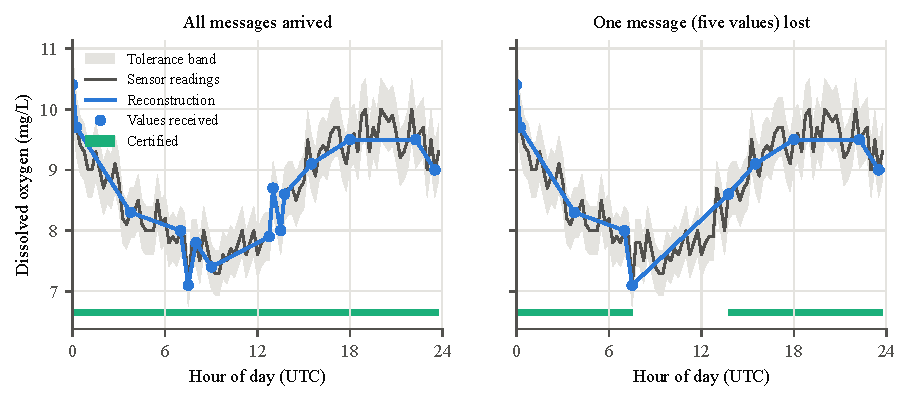
\includegraphics[width=\textwidth]{figs/example_day.pdf}
\caption{Dissolved oxygen on 1 July 2023 at a development site: the record (15 values in three messages) keeps every reading within tolerance; when the middle message is lost, the server certifies the readings outside the gap (bar) and leaves the gap uncertified.}
\label{fig:example}
\end{figure}

\begin{table}[t]
\centering
\caption{Environmental decisions at six messages per day (confirmation sites, four-parameter days). Decided: certainly exceeded or certainly not. Missed: exceedance days that the reconstruction, read naively, did not show.}
\label{tab:env}
\small
\begin{tabularx}{\textwidth}{@{}>{\raggedright\arraybackslash}X*{4}{>{\raggedright\arraybackslash}p{2.2cm}}@{}}
\toprule
Outcome & Record-first code & Record-first repetition & Every $k$-th reading & Tag practice \\
\midrule
\tableinput{tables/env.tex}
\bottomrule
\end{tabularx}
\end{table}

The record does not resolve features finer than its tolerance. pH exceedances in these data were mostly peaks one or two tenths above 9.0, against a tolerance of 0.2. A record within tolerance may flatten such a peak; therefore, read naively, it missed \missPHConf{} of \eventsPHConf{} pH exceedance days, against \missPHEveryConf{} for every $k$-th reading. The three-valued reading reports these days as undetermined rather than clear. For the same reason, periodic samples located the daily peak of dissolved oxygen and its diel range as well as the record did, or better (development data).

\subsection{Robustness}
\label{sec:robust}
Out-of-range readings were carried as censored flags: with one or three faulty readings injected per day, every day remained certifiable, at a cost of approximately \glitchCostDev{} values per faulty reading. Corruption of arriving messages acted as additional loss: at six messages per day the share of fully certified days fell from \corrNoneConf{} without corruption to \corrBerThreeConf{} at a bit-error rate of $10^{-3}$, with no reading certified outside its tolerance. At a bit-error rate of $10^{-2}$, where only 16\% of messages arrive intact, one corrupted parity message passed the CRC-16 by chance on one day and \falseCertConf{} readings were certified wrongly (Section~\ref{sec:confirm}). Removing record days did not change the bytes of any other day; therefore, outages do not propagate.

\subsection{Computational resources}
\label{sec:resources}
On the development data, the encoder needed a median of \opsFifteenDev{} window updates for a four-parameter day at 15-minute sampling and \opsFiveDev{} at 5 minutes, with memory proportional to the number of readings. Measured in Python on a desktop computer, it took a median of \hostFifteenS{}\,s and \hostFifteenKB{}\,kB of peak memory for a 15-minute day and \hostFiveS{}\,s and \hostFiveKB{}\,kB for a 5-minute day, against \hostTableFiveS{}\,s and \hostTableFiveMB{}\,MB for the reference implementation with a full error table; interpreter overhead dominates these times; therefore, the operation counts are the portable measure. At a conservative 200 processor cycles per update, a 48\,MHz microcontroller would encode a 5-minute day in approximately \mcuFiveDev{}\,s; the module's transmission energy, at most 2.5\,J per message \citep{kineis2023kim1}, exceeds the encoding energy by approximately three orders of magnitude. These figures are estimates; no microcontroller was used.

\subsection{Confirmation and temporal re-test}
\label{sec:confirm}
Six of the eight confirmatory hypotheses were supported (Table~\ref{tab:hyp}). C1 was not supported: the median record was \needMedConf{} bytes, within the predicted two messages, but the upper end of its interval (\needMedConfHi{} bytes) exceeded the 30-byte threshold, because the confirmation sites varied more than the development sites. C2 was not supported: on one of the \nDaysCorrConf{} days of the corruption experiment, at the highest bit-error rate tested, a corrupted parity message passed the CRC-16, an event expected approximately \collisionsExpConf{} times among the \crcChecksConf{} CRC checks of corrupted data at that error rate. The frozen receiver retried its erasure decoding over several parity combinations, and each retry is another chance for a corrupted message to pass a 16-bit check. After the confirmation, a corroboration rule was added: a decoding accepted only after an earlier attempt had failed must reproduce a received message that it did not use. A first attempt was left unchanged because it carries the same single-check risk as any received data unit. In an exploratory re-run of the corruption experiment on both cohorts, this rule removed every false certificate (\falseCertPostConf{} on the confirmation and \falseCertPostDev{} on the development sites) at a cost of \postCostThreeConf{} in the share of fully certified days at a bit-error rate of $10^{-3}$ and nothing without corruption. Under extreme corruption ($10^{-2}$), repetition then certified more days than the code (\postRepTwoConf{} against \postCodeTwoConf{}), because the code rejects decodings that it cannot corroborate.

Two low-cost deployments, opened in an earlier round of this study, were re-analysed after the confirmation as an exploratory check. On the InWaterSense node in Kosovo \citep{ahmedi2022} (\inwsDays{} four-parameter days), the record cost a median of \inwsMedBytes{} bytes, approximately 2.4 times the USGS median, and the code certified \inwsCodeSix{} of days at six messages per day (repetition \inwsRepSix{}) and \inwsCodeTwelve{} at twelve. On the Weija intake in Ghana \citep{adumanu2020} (temperature and conductance, \weijaDays{} days), the record cost \weijaMedBytes{} bytes and the code certified \weijaCodeSix{} of days at six messages per day (repetition \weijaRepSix{}). Noisy low-cost records therefore need larger plans; the small number of days makes these results indicative only.

On the 2024 data of the development sites (temporal re-test), the record-first code certified \gCodeIidRetest{} of days at six messages per day and $p = 0.3$, and the median record was \needMedRetest{} bytes; all eight criteria of Table~\ref{tab:hyp} were met, which is expected for sites whose 2023 data shaped the method and is therefore not counted as confirmation.

\section{Discussion}
\label{sec:discussion}

\subsection{Guidance for monitoring agencies}
The results support five recommendations for remote river monitoring over message-priced, one-way links. They are conditional on the loss models and tolerances studied:
\begin{enumerate}
  \item Send a record within tolerance, not the readings. A four-parameter day needed a median of two 23-byte messages, against at least 47 for the raw readings at 10-minute sampling. Periodic readings and broken-stick points of the same size rarely kept every reading within tolerance and could not be certified.
  \item Protect the whole record and let the node size the code. The record-first code needs no estimate of the loss process and was never worse than any linear design over the same units; repetition is a simpler alternative whose disadvantage is small under long bursts of loss.
  \item Plan for twelve messages per day where loss is bursty. Six messages per day certified most days under independent loss of 0.3 but met the 90\% target at only a few sites under bursty loss; twelve met it at almost every site under both.
  \item Choose the plan from a pilot that includes the active season. A 28-day pilot chose an adequate plan for most site-pilots, but winter pilots underestimated the summer need.
  \item Use certified readings for decisions and report undetermined days as such. Certain decisions were never wrong; near-threshold quantities and diel shape need a tighter tolerance or direct samples.
\end{enumerate}

Neither satellite contact time nor energy was the binding constraint. The module draws 500\,mA at 5\,V for less than one second per message \citep{kineis2023kim1}; therefore, twelve messages per day cost at most 30\,J, and encoding costs approximately a thousandth of that. The constraint was the message quota.

\subsection{Relation to earlier work}
The encoder, the code, and the satellite practice are established \citep{imai1988,reed1960,boehme2009}. The findings qualify their combination for one-way links. The design that is optimal when every message arrives \citep{deligiannakis2007} certified few days once messages could be lost, and a code whose dimension is fixed in advance depended on knowing the loss rate, whereas the record-first code did not. Broken-stick telemetry \citep{boehme2009,photopoulou2015} fixes the number of points rather than the accuracy, which is why it rarely met the tolerance; its pseudo-random transmission was a smaller handicap than its content. Rotating a week of data, as satellite tags do, added time diversity under long bursts at the cost of timeliness, which suggests coding across days as a natural extension. The decision analysis connects the framework to the quality-assurance practice of environmental sensing \citep{campbell2013,horsburgh2015}: a certified record states which readings are trustworthy within a known bound, which flagging alone does not.

\subsection{Limitations}
The results carry the following limitations:
\begin{itemize}
  \item Channels: no measured loss process was available for a satellite IoT service; loss rates and burst lengths were swept, and results are conditional on these synthetic channels. Field measurements could narrow the plan recommendation.
  \item Hardware: no satellite module or microcontroller was used; resource figures for a node are estimates from operation counts. The operator's message format and integrity checks were taken from its public documentation \citep{kineis2024formats} and should be confirmed with the operator.
  \item Integrity: certification assumes that the values used arrived as transmitted. A CRC-16 leaves a residual rate of undetected corruption; the confirmation met it once at a bit-error rate of $10^{-2}$, and the corroboration rule adopted afterwards was evaluated only exploratorily. The operator's device identifier is not cryptographic; a message authentication code would cost one value per message.
  \item Sensor accuracy: the tolerance bounds the error added between the sensor and the server, not the error of the sensor; calibration, fouling, and drift remain the task of quality assurance upstream of the encoder.
  \item Clock: the node clock must stay within half a sampling interval of the true time; a typical crystal requires resynchronisation every few months at 5-minute sampling.
  \item Data: the confirmatory evidence comes from USGS-grade instruments in the United States. Low-cost sensors in Kosovo and Ghana were analysed only exploratorily, on \inwsDays{} and \weijaDays{} days; their records cost more and needed larger plans. Tropical rivers affected by mining, which motivated this study, remain to be evaluated with sufficient data.
  \item Decisions: the criteria and thresholds were illustrative of common regulatory practice; agencies use other criteria, and features finer than the tolerance require a tighter tolerance.
\end{itemize}

\section{Conclusions}
\label{sec:conclusion}

This study developed and evaluated a framework that delivers river water-quality records within a stated tolerance over one-way, message-priced satellite links, and that lets the server certify, from the bytes it received, which readings meet the tolerance. On \nSitesConf{} sealed confirmation sites, a four-parameter day needed a median of two 23-byte messages. With six messages per day and an independent loss of 30\%, the record-first code fully certified \gCodeIidConf{} of days without any knowledge of the loss process, more than repetition, a code of fixed dimension, and the transmission practice of satellite tags; with twelve messages per day it certified \gTwelveIidConf{} of days. Certified records never gave a wrong certain decision and detected conductance pulses that periodic and tag telemetry missed, but they do not resolve features finer than the tolerance. Six of eight frozen hypotheses held; the two that did not exposed a record cost slightly more variable than assumed and a residual integrity risk of the 16-bit check under heavy corruption, which a corroboration rule removed in an exploratory re-run.

For agencies that monitor rivers beyond terrestrial networks, the results mean that an accountable continuous record does not require a high-capacity link, provided that the node sends the right values and protects them as a whole, and that the plan is sized from local data. Future work should measure message loss on operational satellite services, run the encoder on field hardware, evaluate low-cost sensors in tropical rivers, tighten the tolerance near decision thresholds, and code across days.

\section*{Software and data availability}
The software that produced every result is described below:
\begin{itemize}
  \item Name of software: river-wq-satellite-records (encoder, message frame, erasure and fountain codes, receiver and certificate, loss channels, analysis scripts, and unit tests).
  \item Developers: Stephen Kwaku Azongo and Kofi Sarpong Adu-Manu.
  \item Contact: Kofi Sarpong Adu-Manu, Department of Computer Science, University of Ghana.
  \item Year first available: 2026.
  \item Hardware required: a standard desktop computer.
  \item Software required: Python 3.13 with NumPy 2.3, pandas 2.3, and Matplotlib 3.10 (exact versions in the repository's requirements file).
  \item Program language: Python.
  \item Program size: approximately \progLines{} lines, with \nTests{} unit tests, including golden byte vectors of the message frame.
  \item Availability and cost: free, under the MIT licence for the code and a CC BY 4.0 licence for the derived data and results; developed at \url{https://github.com/steveAzo/river-wq-satellite-records} and archived on Zenodo \citep{azongo2026code}. The confirmation used the commit tagged confirm2-freeze; its freeze record lists the checksums of the code, the plan, and the sealed data.
\end{itemize}
The repository also holds the cleaned USGS data as used, the plans and freeze records of both confirmation rounds, every result file from which the numbers, tables, and figures of this paper are generated, and a single command for each stage. The USGS data are public \citep{usgs2016nwis}; the raw downloads can be regenerated with the included scripts, and their checksums are recorded. The InWaterSense data are available under a CC BY 4.0 licence \citep{ahmedi2022data}. The Weija data belong to the deployment team and are available from the corresponding author on reasonable request; they are not in the repository.

\section*{CRediT authorship contribution statement}
Kofi Sarpong Adu-Manu: Conceptualization, Supervision, Resources, Writing -- review \& editing. Stephen Kwaku Azongo: Methodology, Software, Formal analysis, Investigation, Data curation, Visualization, Writing -- original draft.

\section*{Declaration of competing interest}
The authors declare that they have no known competing financial interests or personal relationships that could have appeared to influence the work reported in this paper.

\section*{Funding}
This research did not receive any specific grant from funding agencies in the public, commercial, or not-for-profit sectors.

\section*{Acknowledgements}
The authors thank the operators of the USGS National Water Information System, the InWaterSense project, and the Weija deployment team for making their data available.


\bibliographystyle{elsarticle-harv}
\bibliography{refs}

\end{document}
